\chapter{Analyse et Conception}

\section{Introduction}
L'analyse des besoins et la conception architecturale constituent l'étape centrale du génie logiciel. Elle permet de traduire les besoins utilisateurs en spécifications techniques précises via le langage UML. Ce chapitre présente les exigences fonctionnelles et non-fonctionnelles détaillées pour chaque acteur. Il expose la modélisation de la plateforme à l'aide de diagrammes UML (Cas d'utilisation, Classes, Séquence, Activité, Déploiement) et formalise le schéma relationnel de la base de données.

\section{Description des besoins du système}
Le système ManageraHub doit gérer trois profils distincts d'utilisateurs. Pour chacun d'eux, nous avons découpé précisément les fonctionnalités clés requises pour assurer le bon fonctionnement de l'ATS et du réseau social.

\subsection{Besoins fonctionnels}

\subsubsection{Espace Candidat (14 fonctionnalités)}
Le Candidat représente le chercheur d'emploi ou le profil souhaitant développer son réseau. Les fonctionnalités associées sont détaillées dans le tableau \ref{tab:features_candidat}.

\begin{table}[H]
\centering
\small
\begin{tabularx}{\textwidth}{c >{\raggedright\arraybackslash}p{4cm} >{\raggedright\arraybackslash}X}
\toprule
\textbf{\#} & \textbf{Fonctionnalité} & \textbf{Description opérationnelle dans Django} \\
\midrule
1 & S'inscrire & Création de compte avec email unique et vérification de mot de passe. \\
2 & Se connecter & Authentification classique sécurisée. \\
3 & OAuth Google / GitHub (Optionnel) & Connexion rapide via des comptes sociaux de confiance (si configuré). \\
4 & Compléter son profil & Ajout de photo, CV PDF, bio, ville et niveau d'études. \\
5 & Gérer ses certifications & Possibilité d'uploader plusieurs documents de certification. \\
6 & Rechercher des offres & Filtrage multicritère (mots-clés, ville, contrat, domaine). \\
7 & Postuler & Soumission de candidature avec un message facultatif et le CV lié. \\
8 & Suivre ses candidatures & Tableau de bord montrant l'état exact (en attente, refusée, etc.). \\
9 & Publier des posts & Ajout de texte avec support d'images/vidéos dans le feed. \\
10 & Liker des posts & Réaction instantanée (like/unlike) sur les publications du réseau. \\
11 & Commenter & Possibilité de laisser des messages textuels sous chaque post. \\
12 & Rechercher des profils & Recherche globale dans la barre de navigation pour les membres. \\
13 & Suivre des membres & Système de Follow/Unfollow pour s'abonner aux actualités d'autrui. \\
14 & Réinitialiser le mot de passe & Envoi d'un lien sécurisé par e-mail en cas d'oubli. \\
15 & Évaluer ses compétences & Passage d'un quiz interactif de soft-skills et de techniques d'entretien avec enregistrement du score. \\
\bottomrule
\end{tabularx}
\caption{Fonctionnalités détaillées de l'acteur Candidat}
\label{tab:features_candidat}
\end{table}

\paragraph{Spécifications détaillées des fonctionnalités Candidat :}
\begin{enumerate}
    \item \textbf{S'inscrire (Inscription) :} Cette fonction permet à un nouveau visiteur de créer un compte candidat. Le formulaire requiert une adresse e-mail unique, un nom d'utilisateur et un mot de passe fort. Le système effectue des validations d'unicité et de sécurité avant d'enregistrer l'utilisateur en base de données.
    \item \textbf{Se connecter (Authentification) :} Permet à un candidat inscrit de s'authentifier de manière sécurisée en fournissant son adresse e-mail et son mot de passe. Le système utilise les sessions sécurisées de Django pour maintenir la connexion.
    \item \textbf{Authentification sociale (OAuth - Optionnel) :} Offre une alternative d'inscription et de connexion rapide via les comptes Google et GitHub, en s'appuyant sur le package \texttt{django-allauth} (intégré dynamiquement si présent) pour récupérer de manière sécurisée les informations de profil public.
    \item \textbf{Compléter son profil (Profiling) :} Permet au candidat de saisir ses informations professionnelles et personnelles (numéro de téléphone, ville, niveau d'études, expériences, compétences, photo de profil, CV au format PDF et lettre de motivation).
    \item \textbf{Gérer ses certifications (Certifications multiples) :} Une fonctionnalité dédiée permettant au candidat d'importer plusieurs documents ou diplômes de certification pour valoriser son profil auprès des recruteurs.
    \item \textbf{Rechercher des offres d'emploi (Sourcing) :} Le candidat accède à un moteur de recherche interne lui permettant de filtrer les annonces par domaine d'activité, ville de destination, type de contrat (CDI, CDD, Stage, etc.) et niveau d'expérience requis.
    \item \textbf{Postuler à une offre (Application) :} Permet d'envoyer son dossier de candidature (CV, lettre de motivation et un message d'accompagnement textuel) à une offre d'emploi active publiée par une entreprise vérifiée.
    \item \textbf{Suivre le statut de ses candidatures (Tracking) :} Un tableau de bord personnel affiche l'état d'avancement de toutes les candidatures soumises (En attente, En cours d'examen, Entretien planifié, Accepté ou Refusé).
    \item \textbf{Publier des posts (Partage social) :} Permet de rédiger des messages courts, d'y adjoindre des images ou des vidéos de réalisations techniques et d'y associer des hashtags de veille technologique.
    \item \textbf{Liker des posts (Interactions) :} Offre la possibilité d'exprimer son intérêt pour les publications d'autres membres du réseau social en cliquant sur un bouton d'évaluation (J'aime).
    \item \textbf{Commenter des posts (Débat) :} Permet de poster des réponses textuelles sous les publications pour échanger avec la communauté sur des thématiques professionnelles ou techniques.
    \item \textbf{Rechercher des profils (Réseautage) :} Une barre de recherche globale permet de retrouver des camarades de promotion, d'anciens collaborateurs ou des profils d'entreprises par nom ou mot-clé.
    \item \textbf{Suivre d'autres membres (Follow) :} Permet de s'abonner aux actualités de profils ciblés pour recevoir leurs publications directement dans son fil d'actualités personnalisé.
    \item \textbf{Réinitialiser son mot de passe :} En cas de perte, le candidat saisit son adresse e-mail et reçoit un lien à durée de validité limitée pour modifier son mot de passe de manière sécurisée.
    \item \textbf{Évaluer ses compétences (Quiz de compétences) :} Permet au candidat de tester ses connaissances sur les soft-skills et les entretiens à travers un quiz d'évaluation de 8 questions. Le score est calculé instantanément et enregistré dans l'historique de ses résultats.
\end{enumerate}

\subsubsection{Espace Entreprise (12 fonctionnalités)}
L'Entreprise est l'entité recruteuse. Son rôle et ses droits de publication sont assujettis à une validation administrative. Les fonctionnalités sont décrites dans le tableau \ref{tab:features_entreprise}.

\begin{table}[H]
\centering
\small
\begin{tabularx}{\textwidth}{c >{\raggedright\arraybackslash}p{4cm} >{\raggedright\arraybackslash}X}
\toprule
\textbf{\#} & \textbf{Fonctionnalité} & \textbf{Description opérationnelle dans Django} \\
\midrule
1 & S'inscrire administrativement & Saisie du nom, de la taille, de l'ICE (15 chiffres) et du RC. \\
2 & Attendre l'approbation & Compte verrouillé en publication tant que l'admin ne l'a pas validé. \\
3 & Compléter profil entreprise & Ajout de logo, site web, secteur d'activité, adresse physique. \\
4 & Publier une offre & Formulaire complet avec titre, contrat, expérience et salaire. \\
5 & Modifier/Supprimer offre & Mise à jour de l'annonce ou retrait logique du feed public. \\
6 & Activer/Désactiver offre & Option d'archivage temporaire pour stopper les candidatures. \\
7 & Consulter les candidatures & Accès aux profils des candidats ayant postulé à ses offres. \\
8 & Télécharger les CV & Accès direct aux documents d'évaluation (CV PDF, LM). \\
9 & Mettre à jour le statut & Sélection entre : En examen, Entretien planifié, Accepté, Refusé. \\
10 & Rechercher des talents & Consultation publique des profils candidats complétés. \\
11 & Modifier ses infos fiscales & Mise à jour de l'ICE/RC nécessitant une nouvelle revalidation. \\
12 & Tableau de bord statistiques & Visualisation des comptes d'offres actives, total de candidatures, en attente et acceptées. \\
\bottomrule
\end{tabularx}
\caption{Fonctionnalités détaillées de l'acteur Entreprise}
\label{tab:features_entreprise}
\end{table}

\paragraph{Spécifications détaillées des fonctionnalités Entreprise :}
\begin{enumerate}
    \item \textbf{S'inscrire administrativement (Entreprise) :} Formulaire d'inscription spécifique requérant le nom de la société, le numéro fiscal marocain Identifiant Commun de l'Entreprise (ICE - 15 chiffres) et le numéro de Registre du Commerce (RC) pour assurer la légitimité fiscale.
    \item \textbf{Attendre approbation (Vérification administrative) :} Le compte créé est placé par défaut en attente. Une restriction applicative bloque l'accès aux fonctions d'écriture et de publication tant que le profil n'est pas approuvé par l'administrateur.
    \item \textbf{Compléter son profil entreprise :} Permet d'enrichir sa vitrine de recrutement en chargeant le logo officiel de l'entreprise, sa taille salariale, son site internet, sa description et l'emplacement géographique de ses bureaux.
    \item \textbf{Publier une offre d'emploi :} Permet de créer une annonce détaillée en spécifiant le titre du poste, le domaine fonctionnel, le type de contrat (CDI, CDD, etc.), le profil recherché, l'expérience minimale requise et la fourchette salariale proposée.
    \item \textbf{Modifier/Supprimer une offre :} Offre la possibilité de corriger les informations d'une annonce publiée ou de procéder à son retrait logique (soft delete) de l'interface utilisateur.
    \item \textbf{Activer/Désactiver une offre :} Permet de suspendre temporairement une offre d'emploi pour stopper la réception de nouvelles candidatures (par exemple, si le poste est en cours de pourvoi) sans pour autant la supprimer définitivement.
    \item \textbf{Consulter les candidatures reçues :} Accès à une liste centralisée de tous les candidats ayant postulé aux offres de l'entreprise, classés par offre et par date de soumission.
    \item \textbf{Télécharger les documents d'évaluation :} Permet aux recruteurs de visualiser directement dans le navigateur ou de télécharger les CVs et les lettres de motivation au format PDF fournis par les postulants.
    \item \textbf{Mettre à jour le statut de postulation :} L'action centrale du recruteur sur le dossier du candidat. Le statut évolue de "En attente" à "En cours d'examen", puis "Entretien planifié", pour finir par "Accepté" ou "Refusé".
    \item \textbf{Rechercher des profils (Sourcing de talents) :} Permet aux recruteurs d'explorer la base de données publique des candidats complétés et de les filtrer par compétences ou par niveau d'études pour réaliser des approches directes.
    \item \textbf{Modifier ses informations fiscales :} En cas de changement de structure légale, l'entreprise peut soumettre de nouveaux identifiants ICE/RC, ce qui repasse automatiquement le compte en mode attente d'approbation.
    \item \textbf{Consulter le tableau de bord de pilotage (Statistiques) :} Interface analytique montrant des indicateurs clés comme le nombre d'offres actives, le volume total de candidatures reçues, les candidatures en attente de revue et les candidats acceptés.
\end{enumerate}

\subsubsection{Espace Administrateur (10 fonctionnalités)}
L'Administrateur supervise la plateforme et assure la modération ainsi que la validation des comptes (tableau \ref{tab:features_admin}).

\begin{table}[H]
\centering
\small
\begin{tabularx}{\textwidth}{c >{\raggedright\arraybackslash}p{4cm} >{\raggedright\arraybackslash}X}
\toprule
\textbf{\#} & \textbf{Fonctionnalité} & \textbf{Description opérationnelle dans Django} \\
\midrule
1 & Connexion sécurisée & Accès restreint via le portail d'administration Django. \\
2 & Dashboard de vérification & Liste des entreprises inscrites en attente de validation légale. \\
3 & Analyser les documents & Examen de l'ICE et du document RC / Modèle J soumis. \\
4 & Approuver l'entreprise & Passage du statut de l'entreprise à "Vérifiée", activant ses droits. \\
5 & Rejeter avec motif & Rejet de l'inscription avec notification pour ICE invalide par exemple. \\
6 & Gérer les utilisateurs & CRUD complet sur les comptes Candidats et Entreprises. \\
7 & Gérer les offres d'emploi & Modération ou suppression d'offres abusives ou mal formatées. \\
8 & Modérer le feed social & Suppression de posts ou de commentaires inappropriés. \\
9 & Journal des actions & Journalisation automatique de toutes les actions (LogEntry). \\
10 & Statistiques d'utilisation & Nombre d'utilisateurs inscrits, d'administrateurs, de comptes actifs et d'entreprises en attente. \\
\bottomrule
\end{tabularx}
\caption{Fonctionnalités détaillées de l'acteur Administrateur}
\label{tab:features_admin}
\end{table}

\paragraph{Spécifications détaillées des fonctionnalités Administrateur :}
\begin{enumerate}
    \item \textbf{Se connecter au panneau d'administration (Django Admin) :} Accès ultra-sécurisé restreint aux seuls comptes disposant du statut de super-utilisateur (\texttt{is\_superuser} et \texttt{is\_staff}).
    \item \textbf{Consulter le dashboard de vérification :} Un écran dédié qui liste chronologiquement les entreprises nouvellement inscrites dont le profil n'a pas encore été analysé et validé par un modérateur.
    \item \textbf{Analyser la conformité légale :} Le modérateur examine l'ICE à 15 chiffres fourni et compare le Registre du Commerce téléchargé avec les données publiques de l'OMPIC pour s'assurer que la société existe officiellement.
    \item \textbf{Approuver l'entreprise (Activation) :} Le modérateur clique sur le bouton de validation, ce qui passe le booléen \texttt{is\_approved} du profil de l'entreprise à \texttt{True}, déverrouillant instantanément l'ensemble de ses fonctionnalités d'écriture.
    \item \textbf{Rejeter la candidature de l'entreprise :} En cas d'incohérence dans l'ICE ou de document RC illisible, l'administrateur rejette le dossier et saisit un motif qui sera envoyé par e-mail à l'entreprise pour lui demander des corrections.
    \item \textbf{Gérer les utilisateurs (CRUD) :} L'administrateur dispose de droits d'édition, de désactivation ou de suppression définitive sur l'ensemble des comptes (Candidats et Recruteurs) pour faire respecter les conditions d'utilisation.
    \item \textbf{Modérer et réguler les offres d'emploi :} Droit de modifier ou de supprimer immédiatement toute offre d'emploi contenant des propos inappropriés, discriminatoires ou ne respectant pas les standards de la plateforme.
    \item \textbf{Modérer le feed social : } Possibilité de supprimer des publications (posts), des images ou des commentaires du réseau social signalés par la communauté comme hors-sujet ou injurieux.
    \item \textbf{Consulter les logs d'activité (Audit) :} Accès aux tables de journalisation (\texttt{LogEntry}) qui enregistrent l'historique complet de toutes les actions effectuées par les modérateurs et administrateurs.
    \item \textbf{Suivre les indicateurs clés de la plateforme :} Un tableau de bord décisionnel regroupant le nombre total d'utilisateurs inscrits, le nombre d'administrateurs, le nombre d'utilisateurs actifs et le volume d'entreprises en attente de vérification.
\end{enumerate}

\subsection{Besoins non-fonctionnels}
Ces besoins garantissent la qualité technique, la robustesse et la pérennité de l'application :
\begin{itemize}
    \item \textbf{Sécurité :} Hashage des mots de passe avec l'algorithme PBKDF2 de Django, protection systématique contre le CSRF sur tous les formulaires (via \texttt{\% csrf\_token \%}), échappement automatique du HTML pour éviter les injections de scripts intersites (XSS), et requêtes ORM paramétrées pour bloquer les injections SQL.
    \item \textbf{Performance et scalabilité :} Optimisation du temps de réponse de la base de données. En développement, l'ORM Django doit utiliser des méthodes d'optimisation de requêtes (\texttt{select\_related} pour les relations un-à-un/un-à-plusieurs directes comme \texttt{User $\leftrightarrow$ CandidateProfile}, et \texttt{prefetch\_related} pour les relations de type plusieurs-à-plusieurs comme les commentaires et les likes de posts).
    \item \textbf{Ergonomie et responsive design :} La charte graphique doit s'adapter de manière fluide sur smartphone (mobile), tablette et ordinateur de bureau (desktop) en assurant le centrage complet de tous les boutons de formulaire, des tableaux de bord et du feed social.
    \item \textbf{Conformité légale :} Protection des données personnelles des candidats (gestion RGPD\allowbreak/Loi 09-08 marocaine) en permettant la suppression de compte et en protégeant les dossiers médias (CVs) de l'accès public direct.
\end{itemize}

\subsection{Outils de développement choisis}
\begin{itemize}
    \item \textbf{Python (version 3.9) :} Langage principal choisi pour sa flexibilité, sa syntaxe concise et sa compatibilité optimale avec l'environnement de production.
    \item \textbf{Django (version 4.2 LTS) :} Framework de développement web backend choisi pour sa robustesse, sa gestion aisée de l'ORM, sa sécurité intégrée et sa structure MVT.
    \item \textbf{MySQL (via PyMySQL) / MariaDB :} SGBD relationnel robuste utilisé en phase de développement local et en environnement cible, configuré pour garantir une intégrité transactionnelle totale.
    \item \textbf{django-allauth (Optionnel) :} Module d'authentification tiers prêt à l'emploi permettant de gérer les flux OAuth (Google et GitHub) de manière optionnelle lorsque le module est présent (\texttt{HAS\_ALLAUTH}).
    \item \textbf{Pillow :} Bibliothèque indispensable pour la manipulation et la validation des formats d'images (logos d'entreprises, avatars candidats).
\end{itemize}


\section{Modélisation UML}

\subsection{Diagramme de cas d'utilisation global}
Le diagramme suivant (figure \ref{fig:uc_global_pfa2}) présente les interactions de tous les acteurs (Candidat, Entreprise, Administrateur) avec les fonctionnalités principales du système :

\begin{figure}[H]
\centering
\resizebox{0.95\textwidth}{!}{
\begin{tikzpicture}[
  actor/.pic={
    \draw[thick, draw=emsiblue, fill=white] (0,0.5) circle (0.2); % Tête
    \draw[thick, draw=emsiblue] (0,0.3) -- (0,-0.25); % Buste
    \draw[thick, draw=emsiblue] (-0.3,0.1) -- (0.3,0.1); % Bras
    \draw[thick, draw=emsiblue] (0,-0.25) -- (-0.2,-0.75); % Jambe gauche
    \draw[thick, draw=emsiblue] (0,-0.25) -- (0.2,-0.75); % Jambe droite
  }
]
    % Acteurs à gauche (alignés verticalement à x = -7.5)
    \pic at (-7.5, 3.5) {actor};
    \node (candidate) at (-7.5, 3.5) [circle, minimum size=1.5cm] {};
    \node (candidate_text) at (-7.5, 2.5) {\textbf{Candidat}};
    
    \pic at (-7.5, 0) {actor};
    \node (company) at (-7.5, 0) [circle, minimum size=1.5cm] {};
    \node (company_text) at (-7.5, -1.0) {\textbf{Entreprise}};
    
    \pic at (-7.5, -3.5) {actor};
    \node (admin) at (-7.5, -3.5) [circle, minimum size=1.5cm] {};
    \node (admin_text) at (-7.5, -4.5) {\textbf{Administrateur}};
    
    % Cadre système d'origine
    \draw[thick, emsiblue] (-5, -7) rectangle (5, 7);
    \node[emsiblue, above] at (0, 7) {\textbf{Système ManageraHub}};
    
    % Cas d'utilisation (taille réduite et police tiny)
    \begin{scope}[every node/.style={draw, ellipse, align=center, minimum width=1.6cm, minimum height=0.5cm, inner sep=4.5pt, fill=white, drop shadow, font=\tiny}]
        \node (auth) at (-2.2, 6.0) {S'authentifier};
        
        \node (prof_cand) at (-2.2, 4.8) {Gérer son Profil};
        \node (cert) at (2.2, 4.8) {Gérer les \\ Certifications};
        
        \node (apply) at (-2.2, 3.4) {Rechercher \& \\ Postuler};
        \node (quiz) at (2.2, 3.4) {Passer un \\ Quiz};
        
        \node (track) at (-2.2, 2.0) {Suivre ses \\ candidatures};
        
        \node (social) at (-2.2, 0.6) {Publier \& \\ Interagir};
        \node (media) at (2.2, 0.6) {Ajouter des \\ Médias};
        
        \node (follow) at (-2.2, -0.8) {Suivre des \\ membres};
        \node (job_mgt) at (-2.2, -2.2) {Gérer les \\ Offres};
        \node (app_mgt) at (-2.2, -3.6) {Gérer les \\ Candidatures};
        
        \node (verify) at (-2.2, -5.0) {Valider les \\ Entreprises};
        \node (check) at (2.2, -5.0) {Vérifier les \\ Documents};
        
        \node (moderate) at (-2.2, -6.2) {Modérer le \\ Contenu};
    \end{scope}
    
    % Liaisons acteurs (toutes vers la colonne de gauche x = -2.2)
    \draw (candidate) -- (auth);
    \draw (candidate) -- (prof_cand);
    \draw (candidate) -- (apply);
    \draw (candidate) -- (track);
    \draw (candidate) -- (social);
    \draw (candidate) -- (follow);
    
    \draw (company) -- (auth);
    \draw (company) -- (job_mgt);
    \draw (company) -- (app_mgt);
    \draw (company) -- (prof_cand);
    \draw (company) -- (social);
    
    \draw (admin) -- (auth);
    \draw (admin) -- (verify);
    \draw (admin) -- (moderate);
    
    % Relations include et extends (entre x = 2.2 et x = -2.2)
    \draw[dashed, -Latex] (cert) -- node[above, font=\tiny\bfseries] {$\ll$extend$\gg$} (prof_cand);
    \draw[dashed, -Latex] (quiz) -- node[above, font=\tiny\bfseries] {$\ll$extend$\gg$} (apply);
    \draw[dashed, -Latex] (media) -- node[above, font=\tiny\bfseries] {$\ll$extend$\gg$} (social);
    \draw[dashed, -Latex] (verify) -- node[above, font=\tiny\bfseries] {$\ll$include$\gg$} (check);
\end{tikzpicture}
}
\caption{Diagramme de cas d'utilisation global}
\label{fig:uc_global_pfa2}
\end{figure}

\subsection{Diagramme de classes technique}
La structure statique des données, mappée directement sur les modèles Django du projet, est représentée dans la figure \ref{fig:classes_pfa2} :

\begin{figure}[H]
\centering
\begin{tikzpicture}[scale=0.52, transform shape, classbox/.style={draw, rectangle, align=center, fill=emsiblue!5, drop shadow, rounded corners=2pt}]
    % User
    \node[classbox] (User) at (0, 9) [minimum width=6cm] {
        \textbf{User (django.contrib.auth)} \\ \rule{5.8cm}{0.4pt} \\
        + username : CharField [Unique] \\
        + email : EmailField \\
        + first\_name : CharField \\
        + last\_name : CharField \\
        + date\_joined : DateTimeField \\
        + is\_active : BooleanField \\
        + is\_staff : BooleanField \\
        + is\_superuser : BooleanField
    };
    
    % CandidateProfile
    \node[classbox] (Candidate) at (-6.5, 4) [minimum width=6cm] {
        \textbf{CandidateProfile} \\ \rule{5.8cm}{0.4pt} \\
        + user : OneToOneField \\
        + phone\_number : CharField \\
        + address : CharField \\
        + city : CharField \\
        + country : CharField \\
        + education\_level : CharField [Choices] \\
        + skills : TextField \\
        + experience\_summary : TextField \\
        + headline : CharField \\
        + bio : TextField \\
        + profile\_picture : FileField \\
        + cv\_file : FileField \\
        + cover\_letter\_file : FileField
    };
    
    % CandidateCertification
    \node[classbox] (Cert) at (-6.5, -1.5) [minimum width=5.5cm] {
        \textbf{CandidateCertification} \\ \rule{5.3cm}{0.4pt} \\
        + profile : ForeignKey $\rightarrow$ CandidateProfile \\
        + file : FileField \\
        + uploaded\_at : DateTimeField
    };
    
    % CompanyProfile
    \node[classbox] (Company) at (6.5, 4) [minimum width=6cm] {
        \textbf{CompanyProfile} \\ \rule{5.8cm}{0.4pt} \\
        + user : OneToOneField \\
        + company\_name : CharField \\
        + industry : CharField \\
        + company\_size : CharField \\
        + phone\_number : CharField \\
        + city : CharField \\
        + country : CharField \\
        + website : URLField \\
        + description : TextField \\
        + logo : ImageField \\
        + background\_image : ImageField \\
        + is\_approved : BooleanField \\
        + ice : CharField [15-digits] \\
        + rc\_number : CharField \\
        + legal\_document : FileField
    };
    
    % JobOffer
    \node[classbox] (Job) at (6.5, -2.5) [minimum width=6.2cm] {
        \textbf{JobOffer} \\ \rule{6.0cm}{0.4pt} \\
        + posted\_by : ForeignKey $\rightarrow$ User \\
        + company\_name : CharField \\
        + title : CharField \\
        + city : CharField \\
        + country : CharField \\
        + job\_type : CharField [Choices] \\
        + contract\_type : CharField [Choices] \\
        + experience\_level : CharField [Choices] \\
        + summary : TextField \\
        + salary\_range : CharField \\
        + is\_remote : BooleanField \\
        + is\_active : BooleanField \\
        + posted\_at : DateTimeField
    };
    
    % JobApplication
    \node[classbox] (App) at (0, -2.5) [minimum width=6.2cm] {
        \textbf{JobApplication} \\ \rule{6.0cm}{0.4pt} \\
        + candidate : ForeignKey $\rightarrow$ User \\
        + job\_offer : ForeignKey $\rightarrow$ JobOffer \\
        + full\_name : CharField \\
        + email : EmailField \\
        + phone\_number : CharField \\
        + application\_text : TextField \\
        + cv\_file : FileField \\
        + cover\_letter\_file : FileField \\
        + status : CharField [Choices] \\
        + submitted\_at : DateTimeField \\ \rule{6.0cm}{0.4pt} \\
        + progress\_steps : Property [List] \\
        + live\_activity\_logs : Property [List]
    };
    
    % QuizResult
    \node[classbox] (Quiz) at (6.5, -7.5) [minimum width=5.5cm] {
        \textbf{QuizResult} \\ \rule{5.3cm}{0.4pt} \\
        + candidate : ForeignKey $\rightarrow$ User \\
        + score : PositiveIntegerField \\
        + total : PositiveIntegerField \\
        + taken\_at : DateTimeField \\ \rule{5.3cm}{0.4pt} \\
        + percent : Property [Int]
    };
    
    % Post
    \node[classbox] (Post) at (-6.5, -5.5) [minimum width=5.5cm] {
        \textbf{Post} \\ \rule{5.3cm}{0.4pt} \\
        + author : ForeignKey $\rightarrow$ User \\
        + content : TextField \\
        + image : FileField \\
        + video : FileField \\
        + location : CharField \\
        + tagged\_company : ForeignKey \\
        + tagged\_users : ManyToManyField \\
        + likes : ManyToManyField \\
        + created\_at : DateTimeField
    };
    
    % Comment
    \node[classbox] (Comment) at (-6.5, -9.5) [minimum width=5cm] {
        \textbf{Comment} \\ \rule{4.8cm}{0.4pt} \\
        + post : ForeignKey $\rightarrow$ Post \\
        + author : ForeignKey $\rightarrow$ User \\
        + content : TextField \\
        + created\_at : DateTimeField
    };
    
    % Follow
    \node[classbox] (Follow) at (0, 4.5) [minimum width=4cm] {
        \textbf{Follow} \\ \rule{3.8cm}{0.4pt} \\
        + follower : ForeignKey $\rightarrow$ User \\
        + following : ForeignKey $\rightarrow$ User \\
        + created\_at : DateTimeField
    };

    % Liaisons avec cardinalités
    \draw[thick, -{Stealth}] (Candidate) -- (User) node[midway, left] {\small 1..1};
    \draw[thick, -{Stealth}] (Company) -- (User) node[midway, right] {\small 1..1};
    \draw[thick, -{Stealth}] (Cert) -- (Candidate) node[midway, left] {\small *..1};
    \draw[thick, -{Stealth}] (App) -- (User) node[midway, left] {\small *..1};
    \draw[thick, -{Stealth}] (App) -- (Job) node[midway, above] {\small *..1};
    \draw[thick, -{Stealth}] (Job) -- (User) node[midway, right] {\small *..1};
    \draw[thick, -{Stealth}] (Quiz) -- (User) node[midway, right, pos=0.8] {\small *..1};
    \draw[thick, -{Stealth}] (Post) -- (User) node[midway, left] {\small *..1};
    \draw[thick, -{Stealth}] (Comment) -- (Post) node[midway, left] {\small *..1};
    \draw[thick, -{Stealth}] (Comment) -- (User) node[midway, right, pos=0.8] {\small *..1};
    \draw[thick, -{Stealth}] (Follow) -- (User) node[midway, above] {\small *..2};
\end{tikzpicture}
\caption{Diagramme de classes techniques complet}
\label{fig:classes_pfa2}
\end{figure}

\subsection{Diagrammes de séquence}
Les diagrammes de séquence UML permettent de représenter la dimension dynamique du système en détaillant chronologiquement les interactions entre les acteurs (utilisateurs) et les différents objets ou composants logiciels de la plateforme ManageraHub lors de l'exécution de cas d'utilisation clés. Pour répondre aux exigences de complétude fonctionnelle, nous présentons ici cinq scénarios critiques.

\subsubsection{1. Inscription et vérification administrative d'une Entreprise}
Ce diagramme (figure \ref{fig:seq_verify_pfa2}) détaille le flux d'inscription administrative d'une entreprise recruteuse et sa validation ultérieure par l'administrateur de la plateforme. Tant que le booléen \texttt{is\_approved} est faux, les droits de publication restent verrouillés :

\begin{figure}[H]
\centering
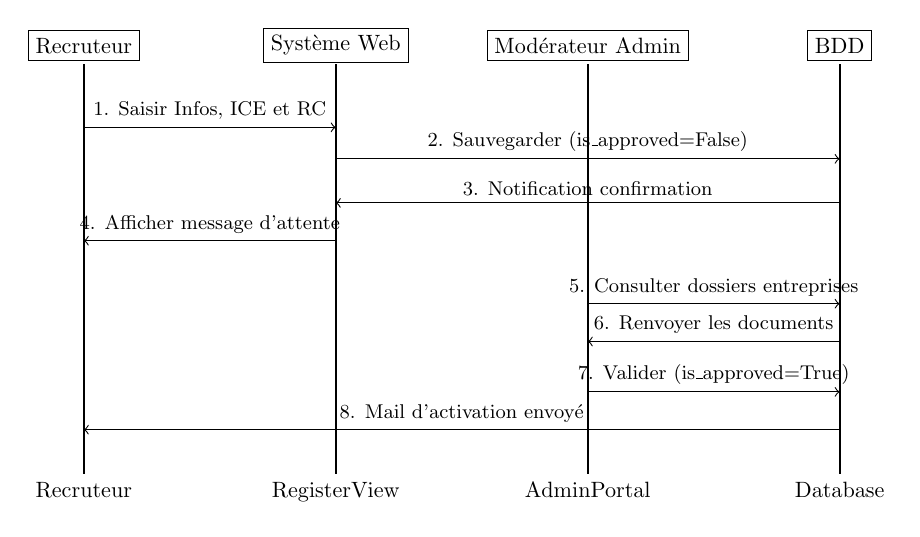
\begin{tikzpicture}[scale=0.8, transform shape]
    % Lignes de vie
    \draw[thick] (0,0) -- (0,-6.5) node[below] {Recruteur};
    \draw[thick] (4,0) -- (4,-6.5) node[below] {RegisterView};
    \draw[thick] (8,0) -- (8,-6.5) node[below] {AdminPortal};
    \draw[thick] (12,0) -- (12,-6.5) node[below] {Database};
    
    \node[draw, fill=white] at (0,0.3) {Recruteur};
    \node[draw, fill=white] at (4,0.3) {Système Web};
    \node[draw, fill=white] at (8,0.3) {Modérateur Admin};
    \node[draw, fill=white] at (12,0.3) {BDD};
    
    % Messages
    \draw[->] (0,-1) -- (4,-1) node[midway, above] {\small 1. Saisir Infos, ICE et RC};
    \draw[->] (4,-1.5) -- (12,-1.5) node[midway, above] {\small 2. Sauvegarder (is\_approved=False)};
    \draw[<-] (4,-2.2) -- (12,-2.2) node[midway, above] {\small 3. Notification confirmation};
    \draw[->] (4,-2.8) -- (0,-2.8) node[midway, above] {\small 4. Afficher message d'attente};
    
    \draw[->] (8,-3.8) -- (12,-3.8) node[midway, above] {\small 5. Consulter dossiers entreprises};
    \draw[<-] (8,-4.4) -- (12,-4.4) node[midway, above] {\small 6. Renvoyer les documents};
    \draw[->] (8,-5.2) -- (12,-5.2) node[midway, above] {\small 7. Valider (is\_approved=True)};
    \draw[->] (12,-5.8) -- (0,-5.8) node[midway, above] {\small 8. Mail d'activation envoyé};
\end{tikzpicture}
\caption{Diagramme de séquence : Inscription et Vérification de l'Entreprise}
\label{fig:seq_verify_pfa2}
\end{figure}

\subsubsection{2. Soumission d'une candidature par un Candidat}
Ce flux (figure \ref{fig:seq_apply_pfa2}) illustre comment un candidat postule à une offre d'emploi active et comment le dossier de candidature est enregistré en base de données :

\begin{figure}[H]
\centering
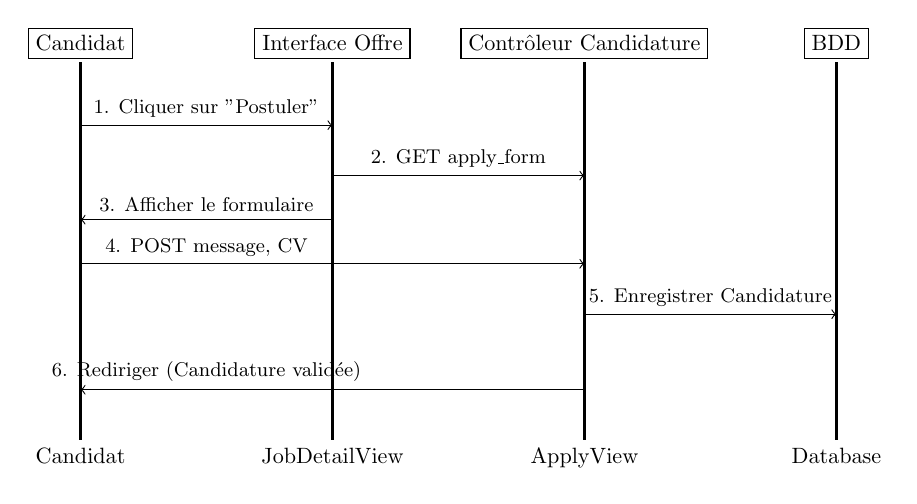
\begin{tikzpicture}[scale=0.8, transform shape]
    \draw[thick] (0,0) -- (0,-6) node[below] {Candidat};
    \draw[thick] (4,0) -- (4,-6) node[below] {JobDetailView};
    \draw[thick] (8,0) -- (8,-6) node[below] {ApplyView};
    \draw[thick] (12,0) -- (12,-6) node[below] {Database};
    
    \node[draw, fill=white] at (0,0.3) {Candidat};
    \node[draw, fill=white] at (4,0.3) {Interface Offre};
    \node[draw, fill=white] at (8,0.3) {Contrôleur Candidature};
    \node[draw, fill=white] at (12,0.3) {BDD};
    
    \draw[->] (0,-1) -- (4,-1) node[midway, above] {\small 1. Cliquer sur "Postuler"};
    \draw[->] (4,-1.8) -- (8,-1.8) node[midway, above] {\small 2. GET apply\_form};
    \draw[<-] (0,-2.5) -- (4,-2.5) node[midway, above] {\small 3. Afficher le formulaire};
    \draw[->] (0,-3.2) -- (8,-3.2) node[midway, above, pos=0.25] {\small 4. POST message, CV};
    \draw[->] (8,-4) -- (12,-4) node[midway, above] {\small 5. Enregistrer Candidature};
    \draw[<-] (0,-5.2) -- (8,-5.2) node[midway, above, pos=0.25] {\small 6. Rediriger (Candidature validée)};
\end{tikzpicture}
\caption{Diagramme de séquence : Flux de candidature}
\label{fig:seq_apply_pfa2}
\end{figure}

\subsubsection{3. Publication d'une offre d'emploi par une Entreprise validée}
Ce scénario (figure \ref{fig:seq_job_pfa2}) montre la cinématique de publication d'une offre. La plateforme vérifie d'abord que le recruteur a été préalablement validé administrativement par le système :

\begin{figure}[H]
\centering
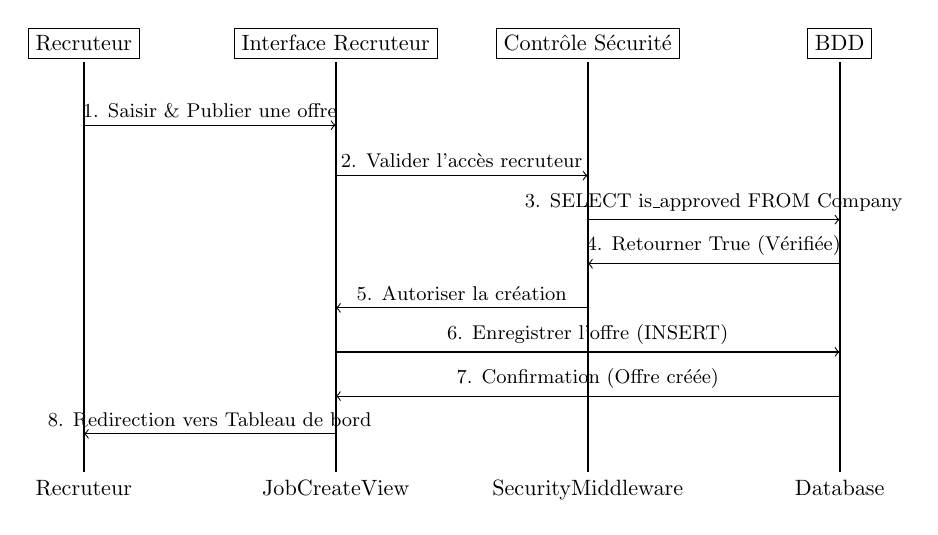
\begin{tikzpicture}[scale=0.8, transform shape]
    % Lignes de vie
    \draw[thick] (0,0) -- (0,-6.5) node[below] {Recruteur};
    \draw[thick] (4,0) -- (4,-6.5) node[below] {JobCreateView};
    \draw[thick] (8,0) -- (8,-6.5) node[below] {SecurityMiddleware};
    \draw[thick] (12,0) -- (12,-6.5) node[below] {Database};
    
    \node[draw, fill=white] at (0,0.3) {Recruteur};
    \node[draw, fill=white] at (4,0.3) {Interface Recruteur};
    \node[draw, fill=white] at (8,0.3) {Contrôle Sécurité};
    \node[draw, fill=white] at (12,0.3) {BDD};
    
    % Messages
    \draw[->] (0,-1) -- (4,-1) node[midway, above] {\small 1. Saisir \& Publier une offre};
    \draw[->] (4,-1.8) -- (8,-1.8) node[midway, above] {\small 2. Valider l'accès recruteur};
    \draw[->] (8,-2.5) -- (12,-2.5) node[midway, above] {\small 3. SELECT is\_approved FROM Company};
    \draw[<-] (8,-3.2) -- (12,-3.2) node[midway, above] {\small 4. Retourner True (Vérifiée)};
    \draw[->] (8,-3.9) -- (4,-3.9) node[midway, above] {\small 5. Autoriser la création};
    \draw[->] (4,-4.6) -- (12,-4.6) node[midway, above] {\small 6. Enregistrer l'offre (INSERT)};
    \draw[<-] (4,-5.3) -- (12,-5.3) node[midway, above] {\small 7. Confirmation (Offre créée)};
    \draw[->] (4,-5.9) -- (0,-5.9) node[midway, above] {\small 8. Redirection vers Tableau de bord};
\end{tikzpicture}
\caption{Diagramme de séquence : Publication d'une offre d'emploi}
\label{fig:seq_job_pfa2}
\end{figure}

\subsubsection{4. Publication de post et interaction (Likes / Commentaires) sur le fil d'actualités}
Ce diagramme (figure \ref{fig:seq_social_pfa2}) modélise le fil d'actualités social, en illustrant la publication d'un contenu par un membre et la réaction instantanée d'un autre utilisateur :

\begin{figure}[H]
\centering
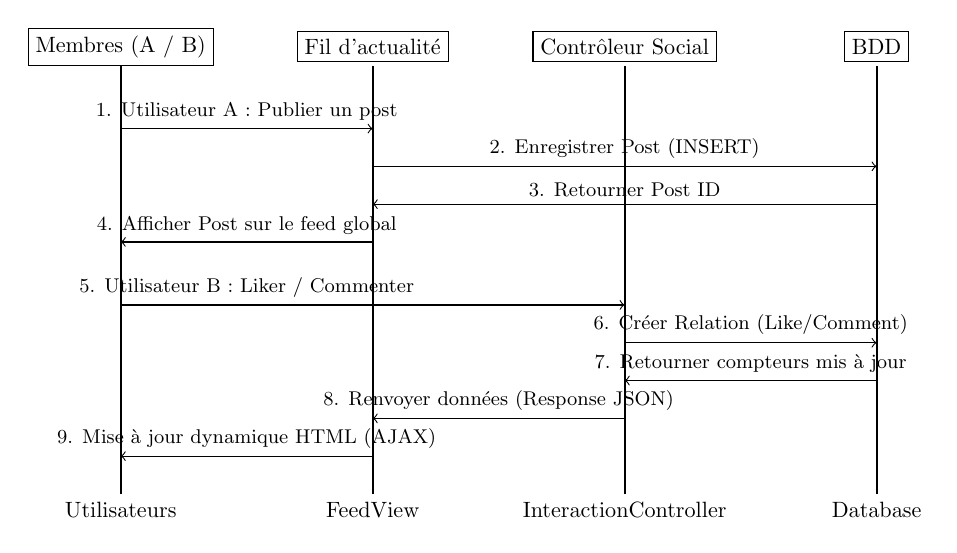
\begin{tikzpicture}[scale=0.8, transform shape]
    % Lignes de vie
    \draw[thick] (0,0) -- (0,-6.8) node[below] {Utilisateurs};
    \draw[thick] (4,0) -- (4,-6.8) node[below] {FeedView};
    \draw[thick] (8,0) -- (8,-6.8) node[below] {InteractionController};
    \draw[thick] (12,0) -- (12,-6.8) node[below] {Database};
    
    \node[draw, fill=white] at (0,0.3) {Membres (A / B)};
    \node[draw, fill=white] at (4,0.3) {Fil d'actualité};
    \node[draw, fill=white] at (8,0.3) {Contrôleur Social};
    \node[draw, fill=white] at (12,0.3) {BDD};
    
    % Messages
    \draw[->] (0,-1) -- (4,-1) node[midway, above] {\small 1. Utilisateur A : Publier un post};
    \draw[->] (4,-1.6) -- (12,-1.6) node[midway, above] {\small 2. Enregistrer Post (INSERT)};
    \draw[<-] (4,-2.2) -- (12,-2.2) node[midway, above] {\small 3. Retourner Post ID};
    \draw[->] (4,-2.8) -- (0,-2.8) node[midway, above] {\small 4. Afficher Post sur le feed global};
    
    \draw[->] (0,-3.8) -- (8,-3.8) node[midway, above, pos=0.25] {\small 5. Utilisateur B : Liker / Commenter};
    \draw[->] (8,-4.4) -- (12,-4.4) node[midway, above] {\small 6. Créer Relation (Like/Comment)};
    \draw[<-] (8,-5.0) -- (12,-5.0) node[midway, above] {\small 7. Retourner compteurs mis à jour};
    \draw[->] (8,-5.6) -- (4,-5.6) node[midway, above] {\small 8. Renvoyer données (Response JSON)};
    \draw[->] (4,-6.2) -- (0,-6.2) node[midway, above] {\small 9. Mise à jour dynamique HTML (AJAX)};
\end{tikzpicture}
\caption{Diagramme de séquence : Interaction fil d'actualités social}
\label{fig:seq_social_pfa2}
\end{figure}

\subsubsection{5. Processus de suivi (Follow / Unfollow) entre membres du réseau}
Le diagramme de la figure \ref{fig:seq_follow_pfa2} modélise l'établissement d'une relation d'abonnement entre deux candidats du réseau social professionnel :

\begin{figure}[H]
\centering
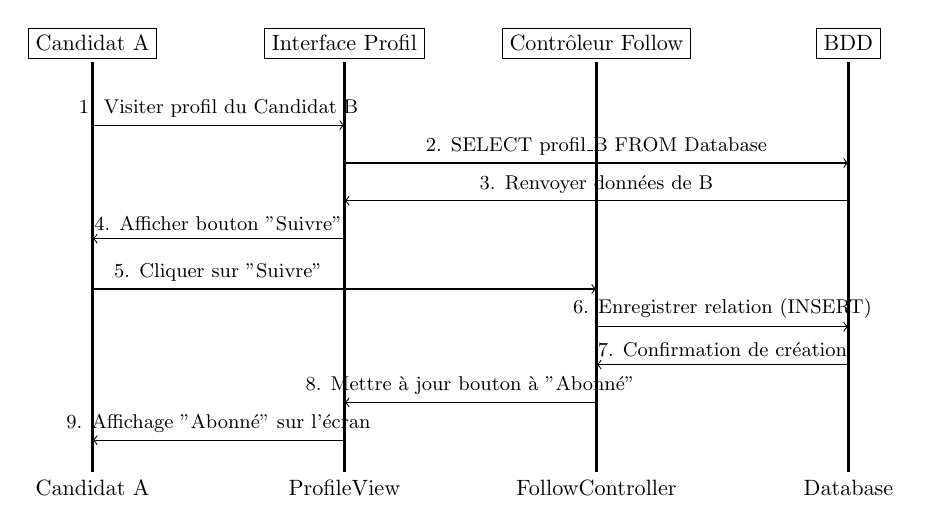
\begin{tikzpicture}[scale=0.8, transform shape]
    % Lignes de vie
    \draw[thick] (0,0) -- (0,-6.5) node[below] {Candidat A};
    \draw[thick] (4,0) -- (4,-6.5) node[below] {ProfileView};
    \draw[thick] (8,0) -- (8,-6.5) node[below] {FollowController};
    \draw[thick] (12,0) -- (12,-6.5) node[below] {Database};
    
    \node[draw, fill=white] at (0,0.3) {Candidat A};
    \node[draw, fill=white] at (4,0.3) {Interface Profil};
    \node[draw, fill=white] at (8,0.3) {Contrôleur Follow};
    \node[draw, fill=white] at (12,0.3) {BDD};
    
    % Messages
    \draw[->] (0,-1) -- (4,-1) node[midway, above] {\small 1. Visiter profil du Candidat B};
    \draw[->] (4,-1.6) -- (12,-1.6) node[midway, above] {\small 2. SELECT profil\_B FROM Database};
    \draw[<-] (4,-2.2) -- (12,-2.2) node[midway, above] {\small 3. Renvoyer données de B};
    \draw[->] (4,-2.8) -- (0,-2.8) node[midway, above] {\small 4. Afficher bouton "Suivre"};
    \draw[->] (0,-3.6) -- (8,-3.6) node[midway, above, pos=0.25] {\small 5. Cliquer sur "Suivre"};
    \draw[->] (8,-4.2) -- (12,-4.2) node[midway, above] {\small 6. Enregistrer relation (INSERT)};
    \draw[<-] (8,-4.8) -- (12,-4.8) node[midway, above] {\small 7. Confirmation de création};
    \draw[->] (8,-5.4) -- (4,-5.4) node[midway, above] {\small 8. Mettre à jour bouton à "Abonné"};
    \draw[->] (4,-6.0) -- (0,-6.0) node[midway, above] {\small 9. Affichage "Abonné" sur l'écran};
\end{tikzpicture}
\caption{Diagramme de séquence : Système d'abonnement (Follow)}
\label{fig:seq_follow_pfa2}
\end{figure}

\subsubsection{6. Suivi en temps réel de statut de candidature (Tracker AJAX)}
Ce diagramme (figure \ref{fig:seq_realtime_pfa2}) modélise le processus d'interrogation en arrière-plan et de synchronisation dynamique du widget de suivi de candidature (Application Tracker) de l'espace candidat. Grâce à des appels AJAX réguliers, les informations de l'historique et de la timeline sont actualisées à la volée :

\begin{figure}[H]
\centering
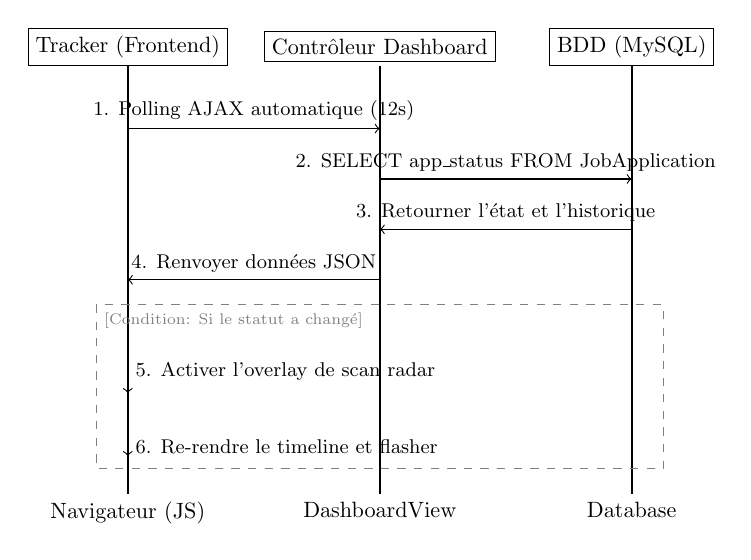
\begin{tikzpicture}[scale=0.8, transform shape]
    % Lignes de vie
    \draw[thick] (0,0) -- (0,-6.8) node[below] {Navigateur (JS)};
    \draw[thick] (4,0) -- (4,-6.8) node[below] {DashboardView};
    \draw[thick] (8,0) -- (8,-6.8) node[below] {Database};
    
    \node[draw, fill=white] at (0,0.3) {Tracker (Frontend)};
    \node[draw, fill=white] at (4,0.3) {Contrôleur Dashboard};
    \node[draw, fill=white] at (8,0.3) {BDD (MySQL)};
    
    % Messages
    \draw[->] (0,-1) -- (4,-1) node[midway, above] {\small 1. Polling AJAX automatique (12s)};
    \draw[->] (4,-1.8) -- (8,-1.8) node[midway, above] {\small 2. SELECT app\_status FROM JobApplication};
    \draw[<-] (4,-2.6) -- (8,-2.6) node[midway, above] {\small 3. Retourner l'état et l'historique};
    \draw[->] (4,-3.4) -- (0,-3.4) node[midway, above] {\small 4. Renvoyer données JSON};
    
    % Condition
    \draw[gray, dashed] (-0.5,-3.8) rectangle (8.5,-6.4);
    \node[gray, anchor=north west] at (-0.5,-3.8) {\scriptsize [Condition: Si le statut a changé]};
    
    \draw[->] (0,-4.5) -- (0,-5.2) node[midway, right] {\small 5. Activer l'overlay de scan radar};
    \draw[->] (0,-5.9) -- (0,-6.2) node[midway, right] {\small 6. Re-rendre le timeline et flasher};
\end{tikzpicture}
\caption{Diagramme de séquence : Synchronisation en temps réel (Tracker)}
\label{fig:seq_realtime_pfa2}
\end{figure}

\subsection{Diagrammes d'activité}

\subsubsection{1. Flux de postulation et mise à jour de statut}
Ce diagramme (figure \ref{fig:act_apply_pfa2}) détaille le cycle de traitement d'une candidature, depuis la recherche d'offre par le candidat jusqu'à la décision finale de recrutement par l'entreprise :

\begin{figure}[H]
\centering
\begin{tikzpicture}[node distance=1.3cm, every node/.style={fill=white, font=\small}, align=center, scale=0.85, transform shape]
    \node (start) [draw, circle, fill=black, inner sep=2pt] {};
    \node (search) [draw, rounded corners, below of=start] {Parcourir et filtrer les offres d'emploi};
    \node (select) [draw, rounded corners, below of=search] {Consulter le détail d'une offre active};
    \node (dec_apply) [draw, diamond, below of=select, aspect=2.2] {Déjà postulé ?};
    \node (error) [draw, rounded corners, right of=dec_apply, xshift=2.5cm] {Afficher message d'erreur \\ (Double postulation interdite)};
    \node (form) [draw, rounded corners, below of=dec_apply, yshift=-0.5cm] {Remplir le message et \\ confirmer l'envoi du CV};
    \node (save) [draw, rounded corners, below of=form] {Enregistrer en BDD \\ (Statut = "En attente")};
    \node (review) [draw, rounded corners, below of=save] {L'entreprise examine le profil \\ (Statut passe à "En cours d'examen")};
    \node (dec_fit) [draw, diamond, below of=review, aspect=2.2] {Profil adéquat ?};
    \node (interview) [draw, rounded corners, below of=dec_fit, yshift=-0.5cm] {Planifier un entretien \\ (Statut = "Entretien")};
    \node (refuse) [draw, rounded corners, right of=dec_fit, xshift=2.5cm] {Notifier le rejet \\ (Statut = "Refusé")};
    \node (dec_final) [draw, diamond, below of=interview, aspect=2.2] {Entretien concluant ?};
    \node (accept) [draw, rounded corners, below of=dec_final, yshift=-0.5cm] {Notifier le recrutement \\ (Statut = "Accepté")};
    \node (end) [draw, double, circle, fill=black!20, below of=accept, inner sep=2pt] {};

    % Liaisons
    \draw[->] (start) -- (search);
    \draw[->] (search) -- (select);
    \draw[->] (select) -- (dec_apply);
    \draw[->] (dec_apply) -- node[above] {Oui} (error);
    \draw[->] (dec_apply) -- node[right] {Non} (form);
    \draw[->] (form) -- (save);
    \draw[->] (save) -- (review);
    \draw[->] (review) -- (dec_fit);
    \draw[->] (dec_fit) -- node[right] {Oui} (interview);
    \draw[->] (dec_fit) -- node[above] {Non} (refuse);
    \draw[->] (interview) -- (dec_final);
    \draw[->] (dec_final) -- node[right] {Oui} (accept);
    \draw[->] (dec_final.east) -- node[above] {Non} ++(1.5,0) |- (refuse.south);
    \draw[->] (accept) -- (end);
    \draw[->] (error.east) -- ++(0.5,0) |- (end.east);
    \draw[->] (refuse.east) -- ++(0.5,0) |- (end.east);
\end{tikzpicture}
\caption{Diagramme d'activité : Processus complet d'une candidature}
\label{fig:act_apply_pfa2}
\end{figure}

\subsection{Diagramme de déploiement}
Ce diagramme (figure \ref{fig:deployment_pfa2}) détaille la topologie physique du déploiement de ManageraHub dans un environnement de production sécurisé :

\begin{figure}[H]
\centering
\resizebox{0.9\textwidth}{!}{
\begin{tikzpicture}[scale=0.85]
    % Navigateur
    \node (browser) [draw, rectangle, minimum width=3.2cm, minimum height=1.6cm, align=center, fill=lightgray] {
        \textbf{Navigateur Client} \\ \rule{3.0cm}{0.4pt} \\
        HTML5 / CSS3 / JS \\
        Moteur Jinja2 (Templates)
    };
    
    % Serveur Applicatif
    \node (appserver) [draw, rectangle, minimum width=4.2cm, minimum height=2.2cm, align=center, fill=emsiblue!10, right=1.2cm of browser] {
        \textbf{Serveur d'Application} \\ \rule{4.0cm}{0.4pt} \\
        Serveur HTTP Nginx \\
        WSGI Gunicorn \\
        \textbf{Framework Django (Python)}
    };
    
    % BDD
    \node (db) [draw, rectangle, minimum width=3.2cm, minimum height=1.6cm, align=center, fill=emsigreen!10, right=1.2cm of appserver] {
        \textbf{Serveur de Données} \\ \rule{3.0cm}{0.4pt} \\
        SGBDR MySQL \\
        Port standard : 3306
    };
    
    % Storage
    \node (storage) [draw, rectangle, minimum width=3.2cm, minimum height=1.6cm, align=center, fill=emsimaroon!10, below=0.8cm of appserver] {
        \textbf{Serveur de Stockage} \\ \rule{3.0cm}{0.4pt} \\
        Répertoire Média \\
        (CVs \& Logos)
    };

    % Connecteurs
    \draw[<->, thick] (browser) -- (appserver) node[midway, above] {\small HTTPS / SSL};
    \draw[<->, thick] (appserver) -- (db) node[midway, above] {\small SQL / Port 3306};
    \draw[<->, thick] (appserver) -- (storage) node[midway, right] {\small I/O Filesystem};
\end{tikzpicture}
}
\caption{Diagramme de déploiement physique du système}
\label{fig:deployment_pfa2}
\end{figure}

\section{Conception de la base de données}

\subsection{Modèle relationnel détaillé}
La base de données relationnelle (MySQL) est structurée pour assurer une intégrité absolue et un temps d'accès optimal. Les tables fondamentales sont listées ci-dessous avec leurs clés primaires (PK) et étrangères (FK) :

\begin{enumerate}
    \item \textbf{auth\_user} \\
    Cette table standard de Django stocke les identifiants de connexion globaux de tous les utilisateurs inscrits.
    \begin{itemize}
        \item \underline{id} [PK] : INT AUTO\_INCREMENT
        \item username : VARCHAR(150) UNIQUE NOT NULL (utilisé pour l'identification et l'URL du profil)
        \item email : VARCHAR(254) NOT NULL
        \item password : VARCHAR(128) NOT NULL (hash sécurisé du mot de passe)
        \item first\_name : VARCHAR(150) NULL
        \item last\_name : VARCHAR(150) NULL
        \item date\_joined : DATETIME NOT NULL
        \item is\_active : BOOLEAN DEFAULT TRUE
        \item is\_staff : BOOLEAN DEFAULT FALSE (TRUE pour les administrateurs)
        \item is\_superuser : BOOLEAN DEFAULT FALSE
    \end{itemize}

    \item \textbf{app1\_candidateprofile} \\
    Stocke les informations personnelles et de profil des chercheurs d'emploi.
    \begin{itemize}
        \item \underline{id} [PK] : INT AUTO\_INCREMENT
        \item \textit{user\_id} [FK $\rightarrow$ auth\_user.id] : INT UNIQUE (relation 1-to-1)
        \item phone\_number : VARCHAR(40) NULL
        \item address : VARCHAR(255) NULL
        \item city : VARCHAR(120) NULL
        \item country : VARCHAR(120) NULL
        \item education\_level : VARCHAR(120) NULL (high\_school, \allowbreak bachelor, \allowbreak master, \allowbreak phd, \allowbreak bootcamp, \allowbreak other)
        \item skills : TEXT NULL
        \item experience\_summary : TEXT NULL
        \item headline : VARCHAR(180) NULL (titre professionnel)
        \item bio : TEXT NULL
        \item profile\_picture : VARCHAR(100) NULL (chemin du fichier avatar)
        \item cv\_file : VARCHAR(100) NULL (chemin du fichier PDF du CV)
        \item cover\_letter\_file : VARCHAR(100) NULL
        \item is\_public : BOOLEAN DEFAULT TRUE
        \item created\_at : DATETIME NOT NULL
        \item updated\_at : DATETIME NOT NULL
    \end{itemize}

    \item \textbf{app1\_candidatecertification} \\
    Gère les certificats multiples importés par le candidat pour appuyer son profil.
    \begin{itemize}
        \item \underline{id} [PK] : INT AUTO\_INCREMENT
        \item \textit{profile\_id} [FK $\rightarrow$ app1\_candidateprofile.id] : INT (relation 1-to-n)
        \item file : VARCHAR(100) NOT NULL
        \item uploaded\_at : DATETIME NOT NULL
    \end{itemize}

    \item \textbf{app1\_companyprofile} \\
    Cette table stocke les données d'identification et les documents légaux de l'entreprise recruteuse.
    \begin{itemize}
        \item \underline{id} [PK] : INT AUTO\_INCREMENT
        \item \textit{user\_id} [FK $\rightarrow$ auth\_user.id] : INT UNIQUE (relation 1-to-1)
        \item company\_name : VARCHAR(180) NOT NULL
        \item industry : VARCHAR(120) NULL
        \item company\_size : VARCHAR(60) NULL
        \item phone\_number : VARCHAR(40) NULL
        \item city : VARCHAR(120) NULL
        \item country : VARCHAR(120) NULL
        \item website : VARCHAR(300) NULL
        \item description : TEXT NULL
        \item logo : VARCHAR(100) NULL
        \item background\_image : VARCHAR(100) NULL
        \item is\_approved : BOOLEAN DEFAULT FALSE (mis à TRUE par l'admin après validation)
        \item ice : VARCHAR(15) UNIQUE NULL (Identifiant Commun de l'Entreprise)
        \item rc\_number : VARCHAR(50) NULL (Registre du Commerce)
        \item legal\_document : VARCHAR(100) NULL
        \item created\_at : DATETIME NOT NULL
        \item updated\_at : DATETIME NOT NULL
    \end{itemize}

    \item \textbf{app1\_joboffer} \\
    Stocke les offres d'emploi publiées par les utilisateurs recruteurs.
    \begin{itemize}
        \item \underline{id} [PK] : INT AUTO\_INCREMENT
        \item \textit{posted\_by\_id} [FK $\rightarrow$ auth\_user.id] : INT NULL
        \item company\_name : VARCHAR(180) NOT NULL
        \item title : VARCHAR(180) NOT NULL
        \item city : VARCHAR(120) NOT NULL
        \item country : VARCHAR(120) NOT NULL
        \item job\_type : VARCHAR(40) NOT NULL (full\_time, part\_time, internship, alternance, freelance, shift)
        \item contract\_type : VARCHAR(40) NOT NULL (cdi, cdd, anapec, stage\_pre, stage\_obs, freelance, ctt)
        \item experience\_level : VARCHAR(40) NOT NULL (junior, mid, senior, lead)
        \item summary : TEXT NOT NULL
        \item responsibilities : TEXT NOT NULL
        \item requirements : TEXT NOT NULL
        \item salary\_range : VARCHAR(120) NULL
        \item is\_remote : BOOLEAN DEFAULT FALSE
        \item is\_active : BOOLEAN DEFAULT TRUE
        \item posted\_at : DATETIME NOT NULL
        \item created\_at : DATETIME NOT NULL
        \item updated\_at : DATETIME NOT NULL
    \end{itemize}

    \item \textbf{app1\_jobapplication} \\
    Gère les dossiers de candidature soumis par les candidats aux offres d'emploi.
    \begin{itemize}
        \item \underline{id} [PK] : INT AUTO\_INCREMENT
        \item \textit{candidate\_id} [FK $\rightarrow$ auth\_user.id] : INT
        \item \textit{job\_offer\_id} [FK $\rightarrow$ app1\_joboffer.id] : INT
        \item full\_name : VARCHAR(180) NOT NULL
        \item email : VARCHAR(254) NOT NULL
        \item phone\_number : VARCHAR(40) NULL
        \item application\_text : TEXT NULL
        \item cv\_file : VARCHAR(100) NULL
        \item cover\_letter\_file : VARCHAR(100) NULL
        \item status : VARCHAR(40) DEFAULT 'sent' (sent, under\_review, accepted, rejected, interview\_scheduled)
        \item submitted\_at : DATETIME NOT NULL
        \item updated\_at : DATETIME NOT NULL
    \end{itemize}

    \item \textbf{app1\_quizresult} \\
    Enregistre les résultats des tests d'évaluation des compétences passés par les candidats.
    \begin{itemize}
        \item \underline{id} [PK] : INT AUTO\_INCREMENT
        \item \textit{candidate\_id} [FK $\rightarrow$ auth\_user.id] : INT NOT NULL
        \item score : INT UNSIGNED NOT NULL
        \item total : INT UNSIGNED NOT NULL
        \item taken\_at : DATETIME NOT NULL
    \end{itemize}

    \item \textbf{app1\_post} \\
    Stocke les messages publiés sur le fil d'actualités social.
    \begin{itemize}
        \item \underline{id} [PK] : INT AUTO\_INCREMENT
        \item \textit{author\_id} [FK $\rightarrow$ auth\_user.id] : INT NOT NULL
        \item content : TEXT NOT NULL
        \item image : VARCHAR(100) NULL
        \item video : VARCHAR(100) NULL
        \item location : VARCHAR(255) NULL
        \item \textit{tagged\_company\_id} [FK $\rightarrow$ app1\_companyprofile.id] : INT NULL
        \item created\_at : DATETIME NOT NULL
    \end{itemize}

    \item \textbf{app1\_comment} \\
    Stocke les commentaires sous les posts du fil d'actualités.
    \begin{itemize}
        \item \underline{id} [PK] : INT AUTO\_INCREMENT
        \item \textit{post\_id} [FK $\rightarrow$ app1\_post.id] : INT NOT NULL
        \item \textit{author\_id} [FK $\rightarrow$ auth\_user.id] : INT NOT NULL
        \item content : TEXT NOT NULL
        \item created\_at : DATETIME NOT NULL
    \end{itemize}

    \item \textbf{app1\_follow} \\
    Représente les relations d'abonnement entre les utilisateurs.
    \begin{itemize}
        \item \underline{id} [PK] : INT AUTO\_INCREMENT
        \item \textit{follower\_id} [FK $\rightarrow$ auth\_user.id] : INT NOT NULL
        \item \textit{following\_id} [FK $\rightarrow$ auth\_user.id] : INT NOT NULL
        \item created\_at : DATETIME NOT NULL
    \end{itemize}

    \item \textbf{app1\_post\_tagged\_users} \\
    Table d'association many-to-many pour les mentions d'utilisateurs sur les posts.
    \begin{itemize}
        \item \underline{id} [PK] : INT AUTO\_INCREMENT
        \item \textit{post\_id} [FK $\rightarrow$ app1\_post.id] : INT NOT NULL
        \item \textit{user\_id} [FK $\rightarrow$ auth\_user.id] : INT NOT NULL
    \end{itemize}

    \item \textbf{app1\_post\_likes} \\
    Table d'association many-to-many pour les mentions "J'aime" sur les posts.
    \begin{itemize}
        \item \underline{id} [PK] : INT AUTO\_INCREMENT
        \item \textit{post\_id} [FK $\rightarrow$ app1\_post.id] : INT NOT NULL
        \item \textit{user\_id} [FK $\rightarrow$ auth\_user.id] : INT NOT NULL
    \end{itemize}
\end{enumerate}

\subsection{Contraintes d'intégrité référentielle}
\begin{itemize}
    \item \textbf{Suppression en cascade (ON DELETE CASCADE) :} Si un compte utilisateur \texttt{User} est supprimé, son profil candidat ou entreprise associé est automatiquement détruit. Il en va de même pour les certifications associées à un profil candidat.
    \item \textbf{Contrainte d'unicité de candidature :} Un candidat ne peut pas postuler plusieurs fois à la même offre. Cette contrainte est implémentée via un index unique MySQL sur le couple (\texttt{candidate\_id}, \texttt{job\_offer\_id}).
    \item \textbf{Contrainte d'unicité de Follow :} Un utilisateur ne peut pas suivre plusieurs fois la même entité. Une contrainte unique est configurée sur les champs \texttt{follower\_id} et \texttt{following\_id}.
    \item \textbf{Intégrité des états de candidature :} Le statut d'une candidature (\texttt{status}) doit obligatoirement appartenir au domaine configuré en base : \{\texttt{'sent'}, \texttt{'under\_review'}, \texttt{'accepted'}, \texttt{'rejected'}, \texttt{'interview\_scheduled'}\}.
\end{itemize}

\section{Conclusion}
La phase d'analyse et de conception UML a permis de formaliser précisément le fonctionnement de la plateforme. La transition vers l'implémentation est désormais sécurisée par un schéma de données clair et des spécifications d'enchaînements dynamiques fiables.
\newpage
